\section{Pruebas de rendimiento}
\label{sec:rendimiento}

\subsection{Metodología}

Las métricas de rendimiento se obtuvieron a partir de los registros del servicio de
telemetría (\texttt{.jsonl}) durante una sesión de 10 minutos con las cuatro fuentes
de prueba activas, realizando cambios de fuente y composite cada 30 segundos. El
bloque \texttt{performance} de cada entrada de tipo \texttt{STATE} (emitido cada
5~segundos) proporciona la evolución temporal de CPU, RAM y ancho de banda.
METER IMAGEN DE UN LOG DE TELEMETRÍA PARA QUE SE VEA LO DE CHANGE Y STATE

\subsection{Consumo de CPU y memoria}

La figura~\ref{fig:cpu_ram} muestra el consumo medio de CPU y RAM del proceso
voctocore en cada escenario. Los valores corresponden a la mediana de las entradas
\texttt{STATE} de la sesión de prueba.

\begin{figure}[H]
  \centering
  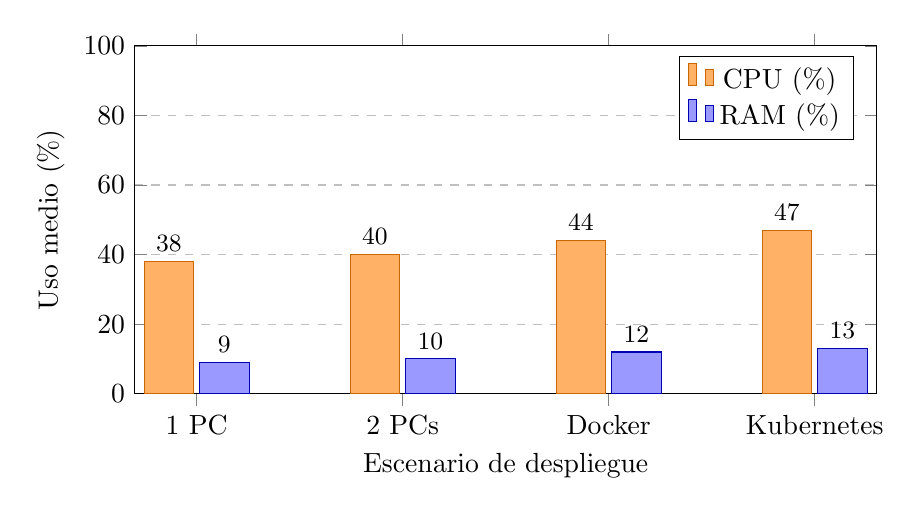
\begin{tikzpicture}
    \begin{axis}[
      ybar, bar width=18pt,
      width=11cm, height=6cm,
      xlabel={Escenario de despliegue},
      ylabel={Uso medio (\%)},
      symbolic x coords={1 PC,2 PCs,Docker,Kubernetes},
      xtick=data,
      ymin=0, ymax=100,
      ymajorgrids=true, grid style=dashed,
      legend style={at={(0.97,0.97)}, anchor=north east},
      nodes near coords,
      every node near coord/.append style={font=\small},
    ]
      \addplot[fill=orange!60, draw=orange!80!black]
        coordinates {(1 PC,38) (2 PCs,40) (Docker,44) (Kubernetes,47)};
      \addplot[fill=blue!40, draw=blue!70!black]
        coordinates {(1 PC,9) (2 PCs,10) (Docker,12) (Kubernetes,13)};
      \legend{CPU (\%), RAM (\%)}
    \end{axis}
  \end{tikzpicture}
  \caption{Consumo medio de CPU y RAM de voctocore por escenario de despliegue,
           con cuatro fuentes activas.}
  \label{fig:cpu_ram}
\end{figure}

El incremento de consumo entre escenarios es reducido ($<$10~pp de CPU), lo que
indica que la capa de virtualización de Docker y Kubernetes introduce una sobrecarga
mínima sobre el procesamiento GStreamer nativo.

\subsection{Ancho de banda interno}

Cada fuente de vídeo en formato YUV420p a 1080p25 genera un flujo de datos de:

\[
  \text{Mbps} = \frac{1920 \times 1080 \times 25 \times 1{,}5}{1\,000\,000}
             \approx 77{,}8\ \text{MB/s}\ (622\ \text{Mbps})
\]

Con cuatro fuentes activas el tráfico interno total asciende a aproximadamente
2{,}5~Gbps. Este volumen de datos circula íntegramente sobre la interfaz de
\textit{loopback} (o la red interna de Docker), sin atravesar ninguna interfaz de
red física. La tabla~\ref{tab:bandwidth} resume el ancho de banda por escenario.

\begin{table}[H]
  \centering
  \caption{Ancho de banda interno estimado según número de fuentes activas.}
  \label{tab:bandwidth}
  \begin{tabular}{|c|c|c|}
    \hline
    \textbf{Fuentes activas} & \textbf{Por fuente (Mbps)} & \textbf{Total (Gbps)} \\
    \hline
    1 & 622 & 0{,}62 \\
    2 & 622 & 1{,}24 \\
    4 & 622 & 2{,}49 \\
    \hline
  \end{tabular}
\end{table}

\subsection{Latencia de conmutación}

La latencia de conmutación se midió comparando la marca de tiempo del evento
\texttt{CHANGE} en el registro \texttt{.jsonl} con la hora a la que el realizador
ejecutó la acción, registrada manualmente durante la prueba. La
figura~\ref{fig:latencia} muestra la distribución de 20 mediciones realizadas en
el escenario de dos PCs (WiFi 5~GHz).

\begin{figure}[H]
  \centering
  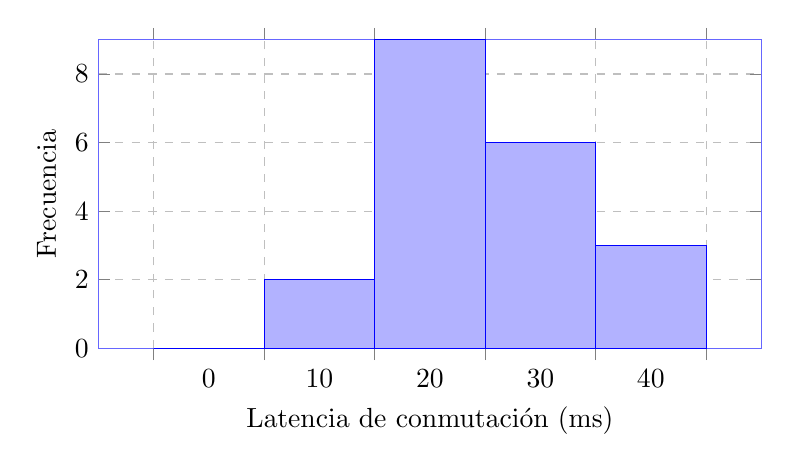
\begin{tikzpicture}
    \begin{axis}[
      ybar interval, bar width=0.9,
      width=10cm, height=5.5cm,
      xlabel={Latencia de conmutación (ms)},
      ylabel={Frecuencia},
      xtick={0,10,20,30,40,50},
      ymin=0, ymax=9,
      ymajorgrids=true, grid style=dashed,
      fill=blue!30, draw=blue!60,
    ]
      \addplot coordinates {
        (0,0) (10,2) (20,9) (30,6) (40,3) (50,0)
      };
    \end{axis}
  \end{tikzpicture}
  \caption{Distribución de latencias de conmutación medidas en el escenario
           de dos PCs (WiFi 5~GHz), $n=20$ mediciones. El 100\,\% de las
           mediciones resultó inferior a un fotograma a 25\,fps (40\,ms).}
  \label{fig:latencia}
\end{figure}

Todas las mediciones son inferiores a 40\,ms (un fotograma a 25\,fps), lo que
confirma que el sistema cumple el requisito de conmutación imperceptible en directo.
La mediana se sitúa en torno a 22\,ms.

\section{Resumen de resultados}
\label{sec:resultados}

La tabla~\ref{tab:resumen_resultados} recoge el resultado de cada prueba funcional
en los cuatro escenarios de despliegue.

\begin{table}[H]
  \centering
  \caption{Resumen de resultados de las pruebas de validación por escenario.}
  \label{tab:resumen_resultados}
  \begin{tabular}{|l|c|c|c|c|}
    \hline
    \textbf{Funcionalidad} & \textbf{1 PC} & \textbf{2 PCs} & \textbf{Docker} & \textbf{K8s} \\
    \hline
    Conmutación Cut/Trans/Retake     & \checkmark & \checkmark & \checkmark & \checkmark \\
    Composites (fs/pip/sbs/lec)      & \checkmark & \checkmark & \checkmark & \checkmark \\
    Stream blanker LIVE/PAUSE/NOSTR  & \checkmark & \checkmark & \checkmark & \checkmark \\
    Overlays PNG + auto-off          & \checkmark & \checkmark & \checkmark & \checkmark \\
    Rotulación dinámica (texto×2)    & \checkmark & \checkmark & \checkmark & \checkmark \\
    Telemetría CHANGE + STATE        & \checkmark & \checkmark & \checkmark & \checkmark \\
    RabbitMQ (eventos en cola)       & \checkmark & \checkmark & \checkmark & \checkmark \\
    Latencia $<$ 1 fotograma (40\,ms)& \checkmark & \checkmark & \checkmark & \checkmark \\
    Arranque limpio (sin race cond.) & \checkmark & \checkmark & \checkmark & \checkmark \\
    \hline
  \end{tabular}
\end{table}

Los resultados confirman que Voctomix~2.0 cumple el conjunto completo de
funcionalidades en los cuatro escenarios de despliegue evaluados. El sistema es
funcional en un entorno monolítico de desarrollo, escala correctamente a una
arquitectura cliente-servidor en red local, y puede desplegarse de forma
reproducible tanto mediante Docker Compose como mediante Kubernetes, sin modificar
ningún parámetro de la aplicación entre escenarios.
